\documentclass[conf]{new-aiaa}
%\documentclass[journal]{new-aiaa} for journal papers
\usepackage[utf8]{inputenc}

\usepackage{graphicx}
\usepackage{amsmath}
\usepackage[version=4]{mhchem}
\usepackage{siunitx}
\usepackage{longtable,tabularx}
\usepackage{float}
\setlength\LTleft{0pt} 

\title{Wii-mote Controlled Graphical User Interface for Crazyflie Drone}

\author{Erika N. Jarosch\footnote{Student}, George V. Petrov\footnote{Student}, Justin L. Roskamp\footnote{Student}, and Kenneth T. Tochihara\footnote{Student}}
\affil{University of Illinois at Urbana-Champaign, Urbana, IL, 61820}

\begin{document}

\maketitle

% Erika
\begin{abstract} 
    The goal of this project is to design and implement a control interface between a Nintendo Wii remote and a Crazyflie 2.0 drone. The Wii Remote serves as an input device to a Windows device via DarwiinRemote. This input is then used with Python package Tkinter to convert Wii remote inputs to positional inputs, which can then be passed through the graphical user interface (GUI). The program interprets the Wii remote inputs and then passes the translated flight plan to the Crazyflie via the input structures developed in the AE 483 course at the University of Illinois at Urbana-Champaign. This goal is motivated by the desire to inspire others with innovative and interactive aerobatics.

\end{abstract}

\section{Nomenclature}
% dynamic- all :)

\section{Introduction}
% Kenneth (v simple, mostly copy)

    The Bitcraze Crazyflie drone and its peripherals provide an accessible, open source platform for custom control development and do-it-yourself projects. \cite{cfclient} With the Crazyradio dongle and Crazyflie Client, it is possible to fly the drone with a standard gaming controller; it is also possible to connect a mobile device directly to the Crazyflie to fly over Bluetooth. However, one can also get closer to the fundamentals of the drone's operation and, as we have done in the AE 483 course, develop custom controllers to perform pre-planned, autonomous flights.
    
    Using this knowledge of custom controls for Crazyflie drones, we sought in this project to develop new methods of interacting with them by using a Wii remote. \cite{darwiin} The Wii remote features an accelerometer and several button. The accelerometer dictates the direction of velocity of the cursor. 
    
    In typical operation, the Wii remote collects data on acceleration, button presses, and pointing, and then it sends this to the Wii console as inputs. The Wii remote sends this data via Bluetooth and is therefore compatible with personal computers when paired with the appropriate software. In this project, the software of intended use is GlovePIE for Windows. This software interprets the Wii remote data as specific mouse and keyboard inputs. These inputs, such as using the infrared camera to move the cursor, make the Wii remote operate in a similar manner to any other input device.
    
    The main mode of operation is to allow the user to draw a flight path with the Wii remote and then send this to the drone such that the drone "copies" the path specified by the user. This requires logging the pointing positions reported by the Wii remote. To accomplish this, the Python package Tkinter is employed. \cite{tkinter} Tkinter's Canvas feature can be made to graphically display a path traced by the cursor, and it allows the binding of events (such as button presses) to functions. For example, one could begin drawing a path by pressing the right mouse button and then end the path by releasing it, similar to Microsoft Paint. The positions describing the path on screen can then be logged automatically. From this, a series of move commands can be crafted and put into a flight plan that the drone can execute.

    On top of the canvas, the GUI features flight control buttons that allow for the user to connect to the drone, run the flight path, abort the flight, and clear the canvas. Furthermore, the user will be able to specify the maximum flight width and the channel number to expand the use case of the application without having to look further into the code. 
    
    While controlling machines with Wii remotes and flying Crazyflies are nothing new in and of themselves, the convergence of these operations does not seem to have been attempted before, and we hope that this unique way of controlling drones can be further developed and used as an outreach tool for the benefit of the fields of study that make this technology possible.

\section{Methods}
% what we used: equations, software and packages

    \subsection{Python Packages}
        
        % tkinter, numpy, time,  (Erika)
        The basis for overall development of the GUI draws heavily upon the tkinter package. Tkinter, an abbreviation for the Tk interface, is the Python interface to the Tcl/Tk GUI toolkit. This toolkit is an amalgam of modules with specific functionalities. Tcl is a dynamic interpreted programming language with a library that utilizes a C interface to command instances of a Tcl interpreter. In tandem with Tkinter, multitasking capabilities are functional via threading. One of the Tcl packages implemented in C, Tk, allowed the group to customize buttons for the interface.
        
        % threading (Kenneth)
        The threading package creates multiple processes. Flags of global variables and objects can be passed in which can change independently from the process created. This makes it possible for flags t o be passed in as global values, allowing for the termination of the function if required. 
        
        % crazyflie client (George)
        
        % gui.py: pixel conversions and normalization set-up (Erika)
        An integral part of the development of the GUI is path normalization from the drawn input to the parameters of the physical room. The pixel width of the square canvas generated by the GUI can be set on the back-end within the gui.py file. The width of the square flight zone can be inputted by the user on the front-end of the GUI, as this may change for a given scenario. These coordinates are given in meters, or 'world coordinates', and are converted into canvas pixels via the "convert\_world\_to\_pixel" function. This function is called when the mouse is clicked on RunFlight, and released. The following equation visualizes how this calculation is made, where x is defined as a given coordinate set:
        \begin{equation}
            X_{Flight} = \frac{X_{World}}{\frac{Canvas Width}{Flight Zone}}
        \end{equation}
        In reality, np.divide is utilized to perform this calculation, and all of the constants are defined through the code. The "convert\_pixel\_to\_world" function completes the opposite conversion, and obtains o\_x and o\_y information to convert to pixel data. This helps to graph the actual flight path from the observer collected coordinates. The np.divide functionality is again utilized for this calculation, and the following equation visualizes how this calculation is made, with x defined as the coordinate set data obtained:
        \begin{equation}
            X_{World} = \frac{X_{Flight}}{\frac{Flight Zone}{Canvas Width}}
        \end{equation}
        
        % client.py:  (Justin)
    
    % client firmware and Wii-mote (George)
    \subsection{Client firmware}
    
    \subsection{Wii-mote}


\section{Design}
% how we implemented code

    % how we used hardware (Justin)
    \subsection{Infrared Sensor Bar}
        
        The original intent of the project was to utilize the Wii Sensor Bar in tandem with the Wii Remote as a positional input system, similar to a mouse. With the Wii, the Sensor Bar allows the user to calibrate a pointing system that can be used to point the remote at specific locations onscreen.
        
        The "Sensor Bar" is a technical misnomer. The bar itself does not do any sensing and is instead an array of passive infrared (IR) LEDs that the Wii Remote senses via an infrared camera on the end of the device. This provides a reference in the field of view of the remote that can be used to determine where the remote is pointing.
        
        In fact, our previous experience with the remote has demonstrated that the Sensor Bar is not required for pointing operations---any appropriately bright infrared source can work, including flames (such as from candles). With this knowledge and the fact that the Wii Sensor Bar has a proprietary connector that is powered via the Wii console, we considered developing or purchasing a USB-powered infrared LED array to simplify the use of our system. Ultimately, this was not required.
        
        Initial testing of the Wii Remote with infrared sources did not appear to provide any positional data to the DarwiinRemote program on macOS. While troubleshooting, we realized that a simpler input method with Wii MotionPlus was possible, and the infrared implementation was effectively abandoned. We believe the infrared approach is possible and worth pursuing in the future, though it was unnecessarily complex in the light of MotionPlus-enabled control. 
    
    \subsection{Wii MotionPlus} % GEORGE HOW THE FUCK DOES GLOVEPIE WORK WITH REMOTE
    
        Wii MotionPlus is an expansion module for the Wii Remote that adds a gyroscope, allowing the controller to detect rotations in addition to linear acceleration and pointing from the built-in accelerometer and IR sensor. Later versions of the Wii Remote, namely the Wii Remote Plus, incorporated the MotionPlus technology inside one device.
        
        As compatibility issues with DarwiinRemote arose with the mid-project upgrade to macOS Monterey, troubleshooting and searches for alternative software led to the use of GlovePIE on Windows 10. % george add here
        
        In our use of GlovePIE and a Wii Remote Plus, two gyroscope measurements are reported: rotation about the remote's longitudinal axis (Y-axis) and about an axis through the side of the remote (X-axis). Rotation about the third axis (the Z-axis, which comes through the face of the remote) is not reported because the MotionPlus gyroscope is dual-axis. In our mapping of the Wii Remote to mouse inputs, pitching the remote upward or downward moves the cursor up or down, while rotating the controller to the left and right moves the cursor left and right, respectively. This configuration is not strictly required, however, and accelerometer measurements, button presses, or additional inputs from devices such as the Wii Nunchuck could be used instead.

    % walk through code set up and implementation
    \subsection{Code Implementation}
    
        Figure \ref{fig:code_logic} describes the user interface logic with the program and considers the many cases in interaction when operating the drone. 
        
        \begin{figure}[H]
            \centering
            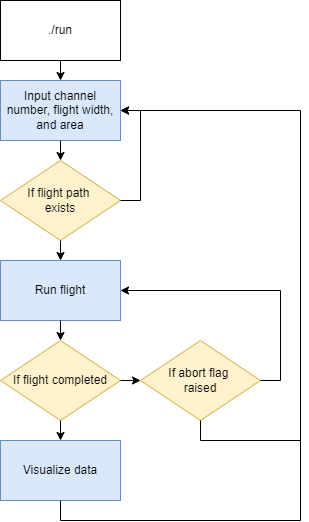
\includegraphics[width=0.4\textwidth]{docs/reports/Final Project Update/images/ae483_code_logic.png}
            \caption{\textbf{GUI with a sample flight drawn.}}
            \label{fig:code_logic}
        \end{figure}
    
        \subsubsection{Python}
            % gui.py (Kenneth)
            The GUI allows for the abstractions of the Crazyflie client controller. Several control functions and the flight path canvas was implemented. One of the flight controller buttons is the Clear button that wipes the canvas and coordinate data. The Connect button establishes connection with the input channel number with the Crazyflie drone. The Run Flight button executes the drawn flight path scaled to the correct width of the flight zone. The Abort button suspends the flight and lands where the drone currently is. 
            
            The main reason for implementation of the Abort button is the concern for safety. If the flight does not seem to go in the correct direction or is on a collision course with another object, the user can hit the abort the button to immediately land the drone. This was critical in the safety of our product, and utilized the threading concepts described previously. The abort flag is raised when the button is pressed, shutting down the function that moves the drone and lands it at the location that the button is pressed at. If the flight is aborted, the flight data will not be visualized and will be reset for the next flight.
            
            The canvas also allows for the user to use a mouse input as a way to draw the desired flight path. The canvas properly checks for cases that are out-of-bounds, and draws appropriately along the boundary of the canvas. The drawn pixels can be then converted to the world coordinates for the drone to fly in. 
            
            % client.py (Erika)
            
            % flight data folder (Kenneth)
            For each flight, a folder is created to add the data after each flight. Utilizing the OS controls, a directory is created based on the date and time the flight concluded. Furthermore, the system takes a snapshot of the screen and saves that file in that same directory. The final data set that saves in that location are the JSON files for the flight data and a PNG file of the GUI interface. This will allow the user to return back to past flights if desired. 
            
            % main.py and run file (Kenneth, ???)
            After creating the GUI and client interface classes, these files were integrated into the main function where everything can be run. The main file allows for the modularization of the different pieces of code and allows for the simplification of running code for the user. A run shell script was also created to abstract the file structure of the repository, and make it easier for the user to start up the GUI. 
        
        \subsubsection{Crazyflie Firmware}
        % custom controller, og observer (George)

\section{Results and Discussion}

    \subsection{Implemented Features}
        % WHAT and WHY functionalities worked/didn't work, iteration (Erika)
        Able to implement some functions like the copy cat and plotting the data on the flight post flight. 
        
        Not able to implement different planes and other modes. 
        
        % Not on mac (Nintendo sux for proprietary software) (George)
    
    % observer traced (Justin)
    \subsection{Observer Results}

        \begin{figure}[H]
        \centering
        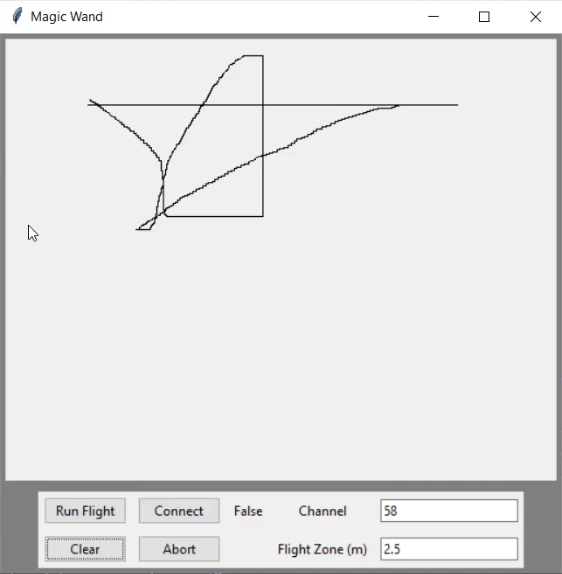
\includegraphics[width=0.6\textwidth]{docs/reports/Final Project Update/images/drawn_flight_path.PNG}
        \caption{\textbf{GUI with a sample flight drawn.}}
        \label{fig:drawn_flight}
        \end{figure}
        
        \begin{figure}[H]
        \centering
        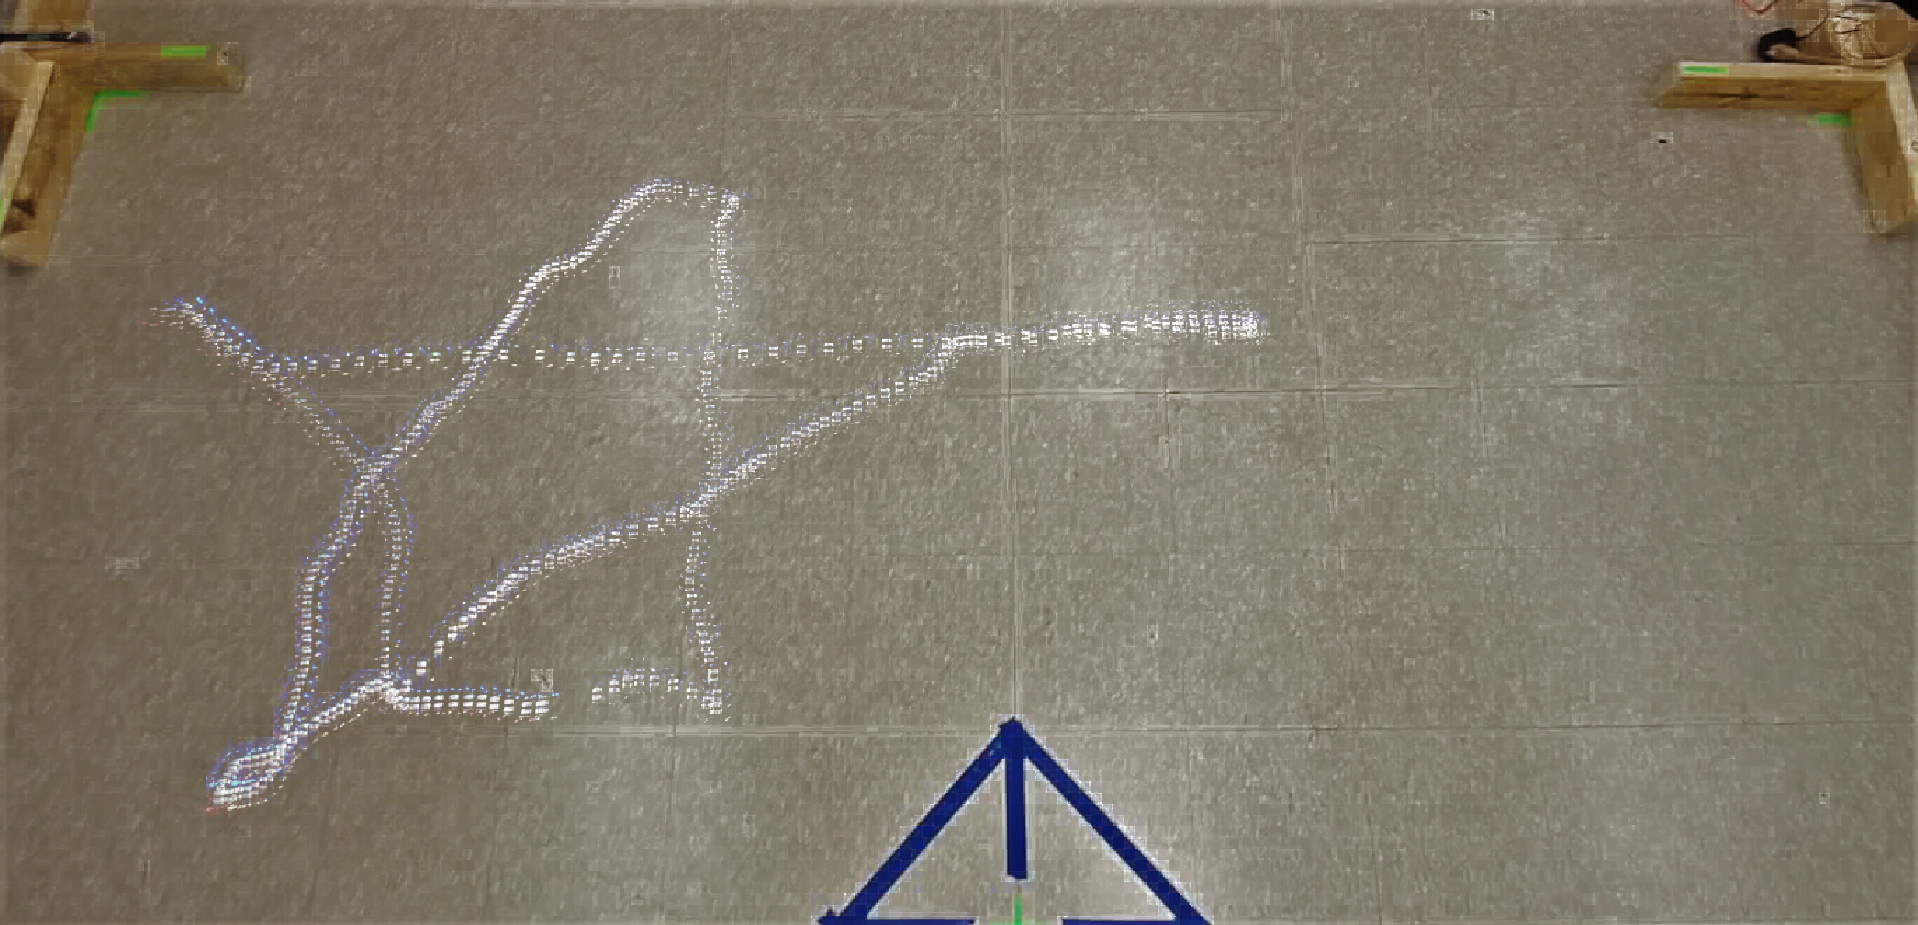
\includegraphics[width=0.6\textwidth]{docs/reports/Final Project Update/images/real_flight_path.png}
        \caption{\textbf{Real-world flight path of sample flight.}}
        \label{fig:drawn_flight}
        \end{figure}

    \subsection{Future Work} % Justin?
    
        Working with other groups to get the light pattering thing to work.
        

\section{Conclusion}
% George

\section{Acknowledgements}
    The authors thank their professor, Tim Bretl; their teaching assistant, Travis Zook; and their laboratory manager, Dan Block.

\appendix

\section{Group Member Contributions} \label{apx:contributions}
    \begin{table}[H]
        \begin{center}
        \setstretch{1}
        \caption{\textbf{Contributions Table}}
        \begin{tabular}{ | p{2in} | p{4in}| } 
            \hline
            \textbf{Group Member} & \textbf{Contribution to Project} \\  \hline
            Erika Jarosch & Flight path code development and interfacing, co-authored Methods, Design, Results, Developed Jupyter Notebook\\ \hline
            George Petrov & Wii Remote implentation, documentation, authored Wii remote section on report\\ \hline
            Justin Roskamp & Interpreted real-world performance and configurations, co-authored Introduction, Design, Results, Conclusion   \\ \hline
            Kenneth Tochihara & GUI and client interface, repository management, documentation, co-authored code-implementation sections on report\\ \hline
        \end{tabular}
        \end{center}
    \end{table}

\section{Code Repository}
    GitHub Repository: \url{https://github.com/ktt3/ae483-magic-wand}



\end{document}